\section{Bayesian PCA}
In this section, an observational study was conducted for Bayesian PCA. Only its most significant aspects related to being a Bayesian representation method were analyzed — some observations were only noted in the last section.

\vspace{\baselineskip}
As a consequence of the characteristics of BPCA (explained throughout this section, and summarized in \nameref{subsec:bpca-conclusions}) for the purpose of the following experiments, the MNIST dataset was reduced to contain 1800 samples of size $8\textrm{x}8$ (firstly, $2$-pixel padding was removed and only then $20\textrm{x}20$ images were scaled down).

\vspace{\baselineskip}
To evaluate the methods reliably, if not stated differently, the following parameters were adopted:
\begin{itemize}
    \item Number of components (PCA) — the result of automatic selection of the corresponding BPCA execution,
    \item number of iterations (BPCA) - $2500$,
    \item gamma distribution hyperparameters (BPCA) — all set to $0.001$.
\end{itemize}

\subsection{Number of principal components}
In conventional PCA, the number of principal components is determined by looking at the cumulative explained variance ratio and arbitrarily setting the cutoff threshold. This implies testing the retained variance for each of the components (or at least a large subset of them). As already mentioned (in the paragraph about \nameref{par:bpca} of \autoref{subsec:pca-theoretical}), BPCA is capable of establishing the number of principal components automatically by estimating the effective dimensionality of the latent space.

\vspace{\baselineskip}
The retrieval of this number can be done in two ways. First, count the nonzero vectors $\mathbf{w}_i$ of the matrix $\mathbf{W}$. Second, it can be inferred directly from $\boldsymbol{\alpha}$ (which is the vector of hyperparameters), because it influences the columns of the said matrix through a conditional distribution $p(\mathbf{W} \mid \boldsymbol{\alpha})$. Both approaches are mathematically related and easily visualizable.

\paragraph{Projection matrix visualization}
The $\mathbf{W}$ matrix can be visualized using a \textit{Hinton diagram}. It is a visualization technique for two-dimensional numerical arrays that represents its values as squares. The color of the square indicates the sign of a number (white represents a positive number, black indicates negative), and the occupied area is proportional to the magnitude of the value.\footnote{The original idea comes from David Warde-Farley on the SciPy Cookbook \cite{Virtanen2020}.}

\vspace{\baselineskip}
The result of fitting the Bayesian PCA model is shown in \autoref{fig:bpca-hinton}. In the Hinton diagram of the projection matrix for the scaled 64-dimensional (images of size $8\text{x}8$) MNIST dataset, 16 zeroed-out columns\footnote{Please note that some vectors' squares of the zeroed-out columns are slightly visible. The cause of this is that the values are not, in fact, equal to $0$. They are considered to be \say{zeroed-out} if they are below a defined threshold (similarly to paragraph \nameref{par:bpca-components-alpha}).} indicate the discarded dimensions. The rest $48$ is thus the number of principal components retained in the model. It will also be treated as a reference in later paragraphs.

% TODO Describe Hinton matrices for 1x10 dataset
\begin{figure}[ht]
    \centering
    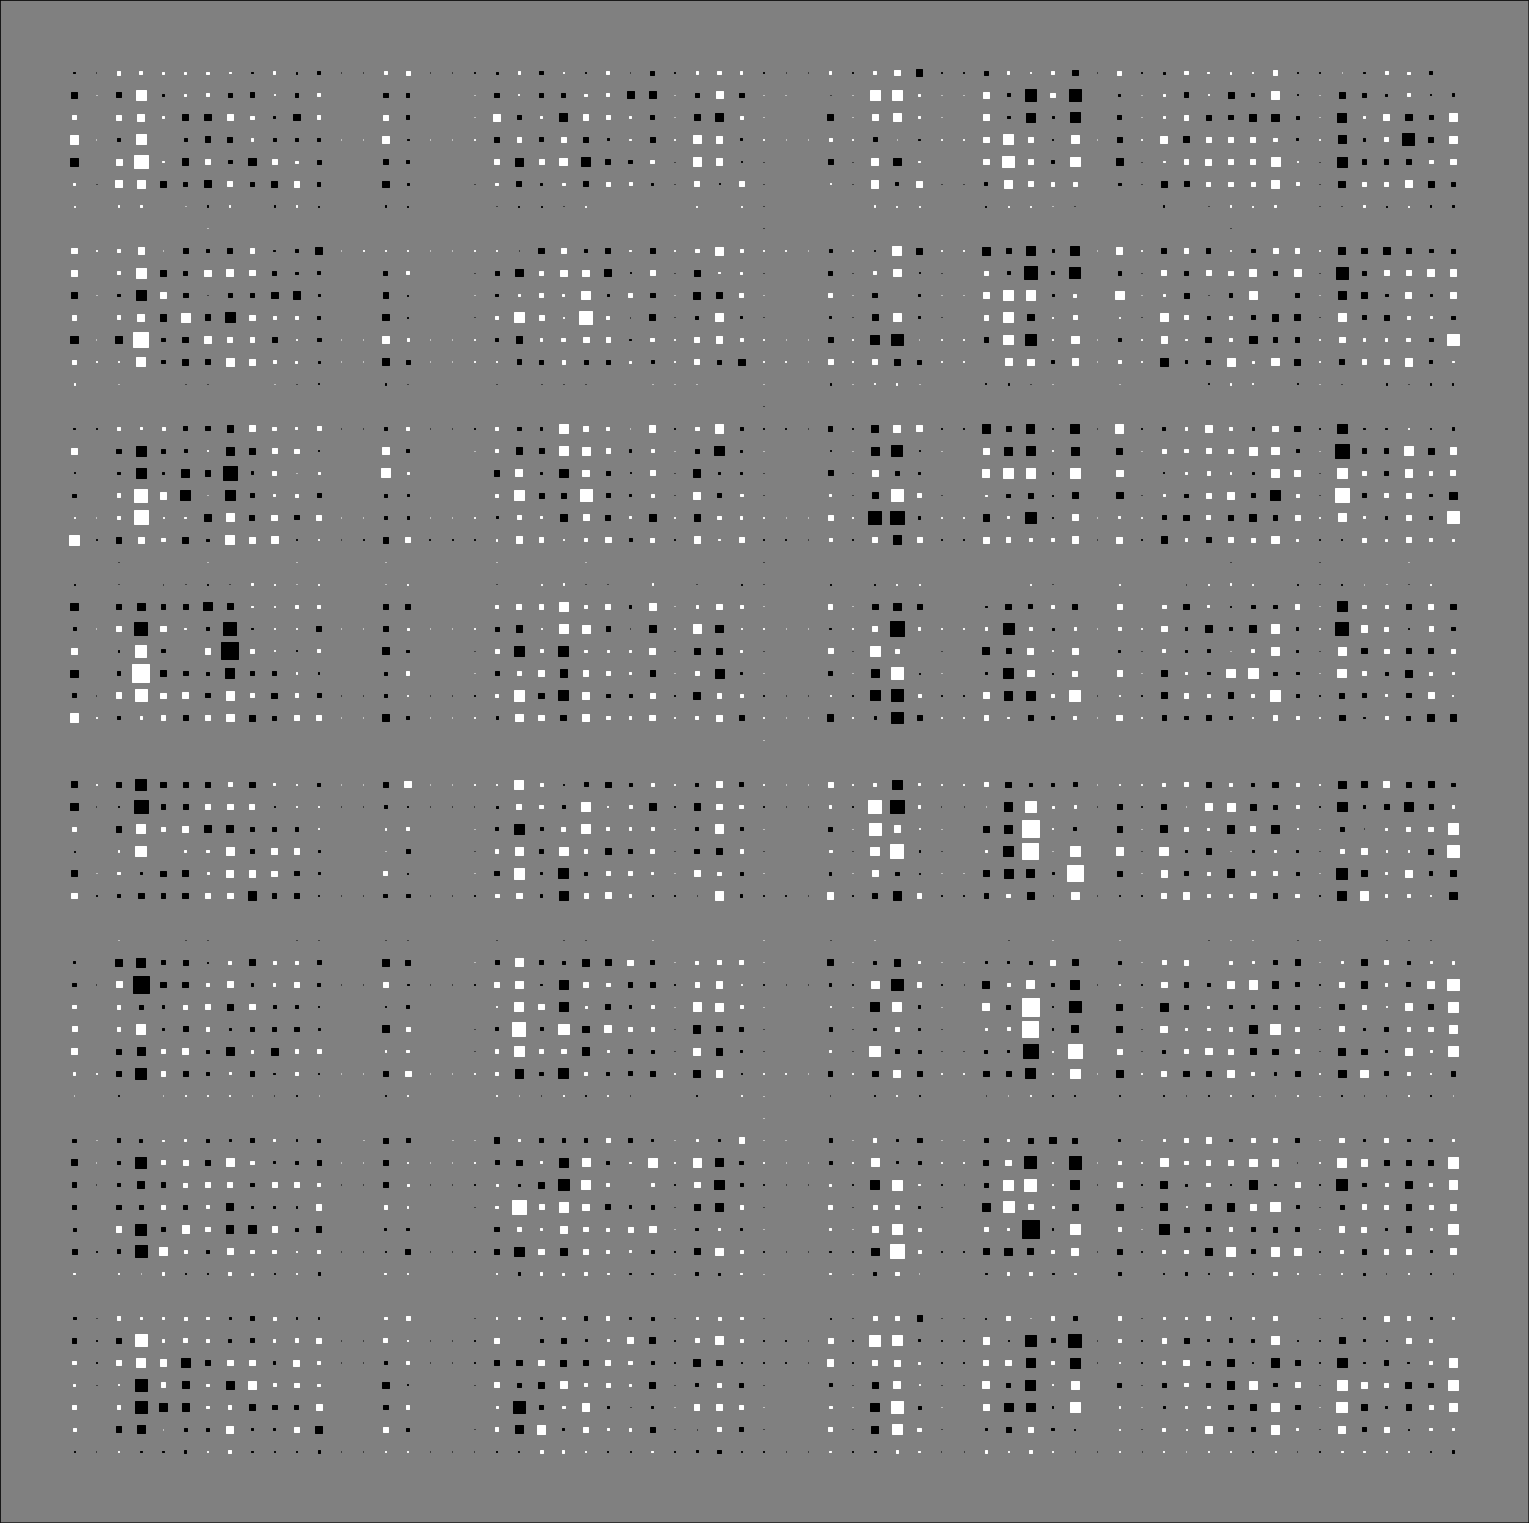
\includegraphics[width=0.9\textwidth]{observational/img/bpca/bpca_hinton_8.png}
    \caption[Hinton diagram of the BPCA projection matrix]{Hinton diagram of the BPCA projection matrix for a MNIST data set in 64 dimensions ($8$x$8$ digits). The model's effective dimensionality, and thus number of principal components, is $q_{eff} = 48$.}
    \label{fig:bpca-hinton}
\end{figure}

% \vspace{\baselineskip}
% Using the same technique, it is also possible to compare the BPCA's $\mathbf{W}$ with the PCA's weight matrix.



\paragraph{Hyperparameter vector $\boldsymbol{\alpha}$}\label{par:bpca-components-alpha}
As already stated, because the columns of the matrix $\mathbf{W}$ are controlled by the $\mathbf{\alpha}$ hyperparameter vector through the conditional distribution, the number of principal components can be inferred directly from it. The \say{zeroing-out} of a weight vector $\mathbf{w}$ (represented by a column in $\mathbf{W}$) occurs when the corresponding $\alpha$ has a large value. Setting a minimum threshold for the values defines the number of principal components (see \autoref{fig:bpca-alpha}).

\begin{figure}[h]
    \centering
    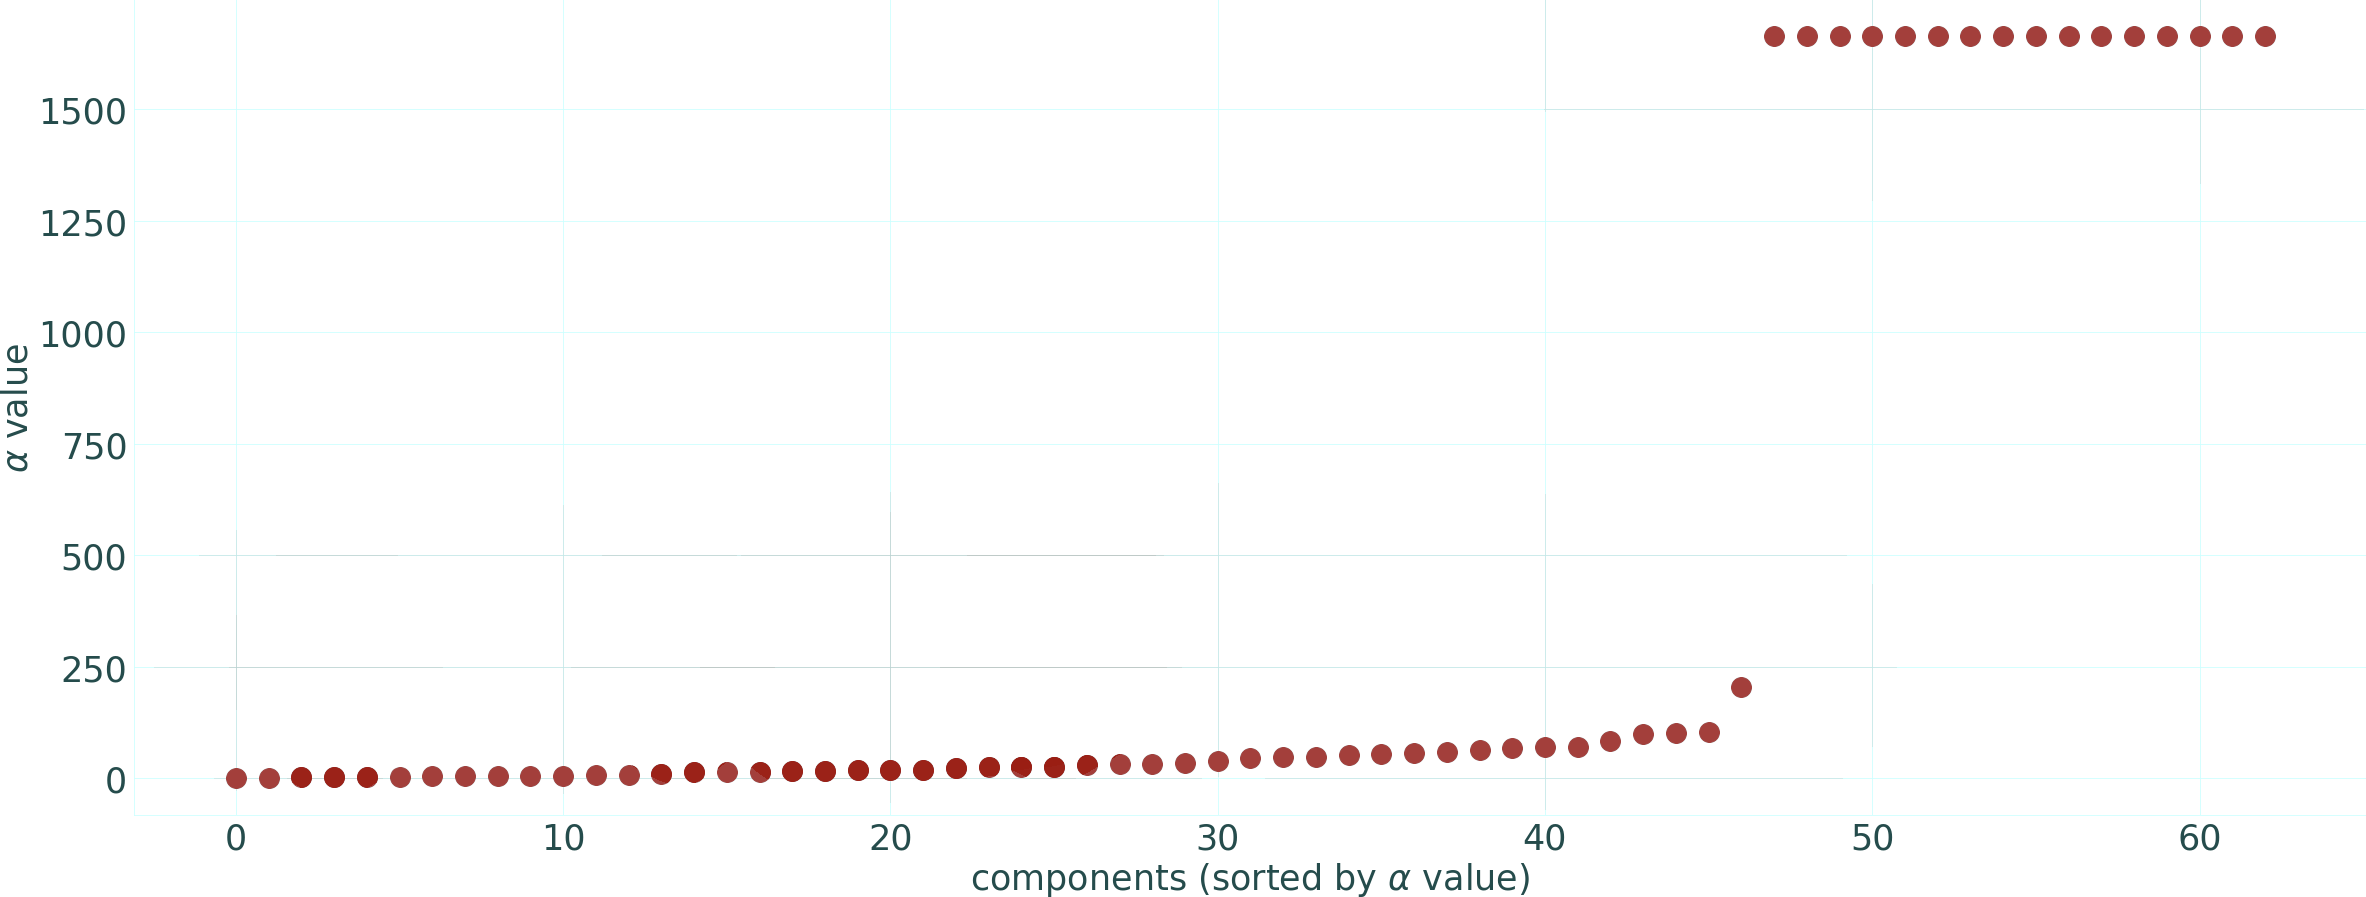
\includegraphics[width=0.9\textwidth]{observational/img/bpca/bpca_alpha.png}
    \caption[Spread of BPCA $\alpha$ hyperparameters]{A spread of the hyperparameters $\alpha$ across components, sorted by their value in a non-decreasing order. Two groups of values are clearly distinguishable - \say{large}, which zero-out columns of the $\mathbf{W}$ matrix, and \say{small}, which correspond with principal components. Note that since the components are sorted by the value of $\alpha$, the number on the x-axis might not necessarily overlap with their number in the search space.}
    \label{fig:bpca-alpha}
\end{figure}

\vspace{\baselineskip}
Due to the reasons mentioned in the previous paragraph, determining the number of principal components of the hyperparameter vector $\boldsymbol{\alpha}$ is more reliable. It is also the approach assumed in most implementations.

\subsection{Inference}
The used implementation of BPCA can track a component that is at the heart of the variational inference framework, \textit{Evidence Lower Bound}. Although it is useful in tracking and evaluating the learning process, it can also provide important information on the underlying uncertainty (as explained in \autoref{subsec:bayesian-inference})

\vspace{\baselineskip}
\autoref{fig:bpca-inference} presents the course of ELBO over the whole learning duration. The graph shows that the learning process stabilizes after $\sim1000-1500$ epochs. Despite fluctuations (which are usually signs of attempts to continue exploring the search space), the plot seems to be approaching a constant asymptote. 

\begin{figure}[h]
     \centering
     \begin{subfigure}[b]{0.9\textwidth}
         \centering
         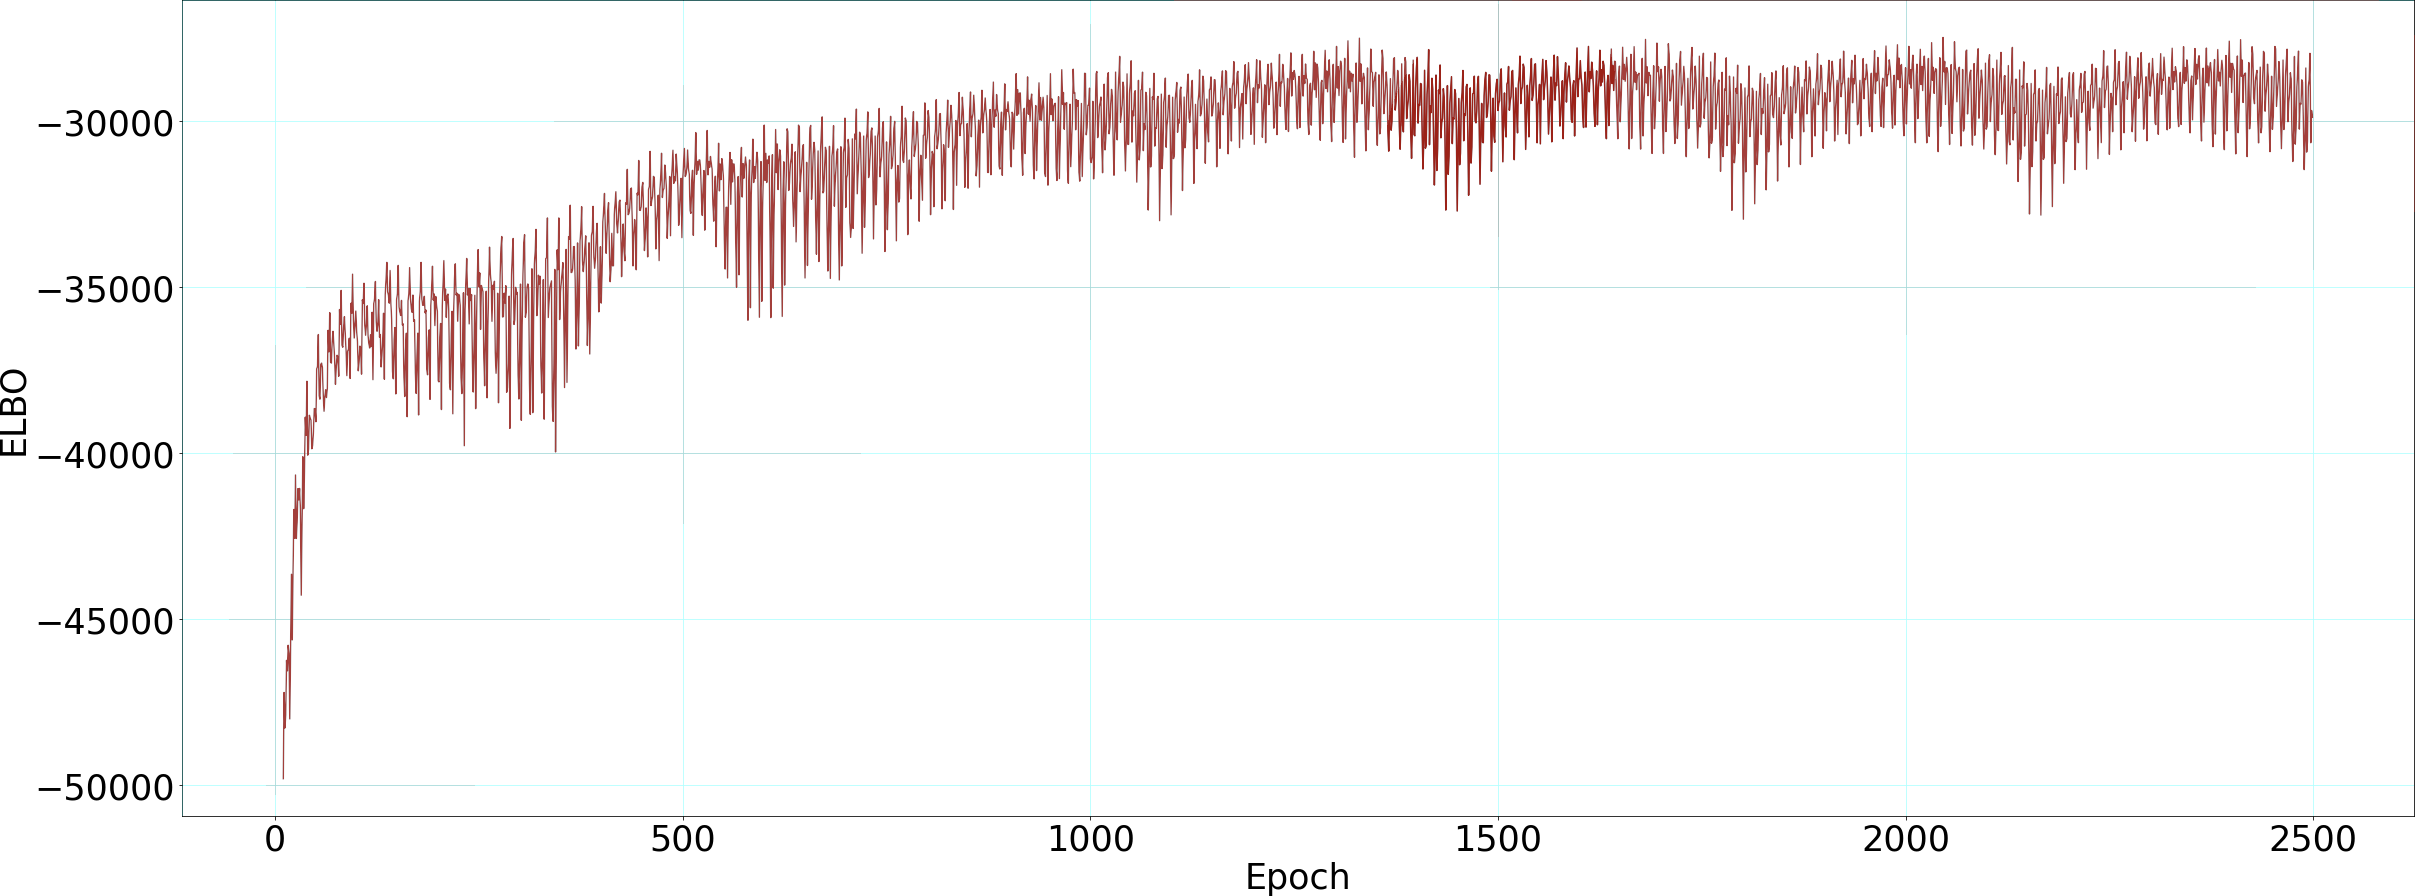
\includegraphics[width=\textwidth]{observational/img/bpca/bpca_elbo.png}
         \caption{ELBO over epochs}
         \label{fig:bpca-inference:loglikelihood}
     \end{subfigure}
     \caption[ELBO course during BPCA inference]{Graph shows Evidence Lower Bound values over model training epochs. Note that first 10 epochs were omitted for better legibility.}
    \label{fig:bpca-inference}
\end{figure}



% \subsection{Captured dimensions}

\subsection{Representation reconstruction}
Both approaches to PCA have the possibility of inverting their transforms. In this manner, reconstruction of the original values is possible, and visual evaluation of the representations is feasible. Visualizations of data reconstruction by PCA and BPCA were presented in \autoref{fig:bpca-reconstruction}.

\begin{figure}[h]
     \centering
     \begin{subfigure}[b]{0.9\textwidth}
         \centering
         
\includegraphics[width=\textwidth]{observational/img/bpca/bpca_reconstruction_original.png}
         \caption{Original data}
     \end{subfigure} 
     \par\bigskip
     \begin{subfigure}[b]{0.9\textwidth}
         \centering
         
\includegraphics[width=\textwidth]{observational/img/bpca/bpca_reconstruction_pca.png}
         \caption{PCA reconstruction}
     \end{subfigure}  
     \par\bigskip
     \begin{subfigure}[b]{0.9\textwidth}
         \centering
         
\includegraphics[width=\textwidth]{observational/img/bpca/bpca_reconstruction_bpca.png}
         \caption{Bayesian PCA reconstruction}
     \end{subfigure} 
     \caption[Reconstruction of data with PCA and BPCA]{Visualizations of data reconstruction with PCA (b) and Bayesian PCA (c).}
    \label{fig:bpca-reconstruction}
\end{figure}

\vspace{\baselineskip}
It can be noticed that while the latter is quite accurate (with only slight smudges around some numbers), the former does not always cope with it correctly. It is especially visible when comparing numbers $7$, $8$, and $9$, where conventional PCA adds artifacts to the background. This is due to either imposing the number of principal components inferred from BPCA, or BPCA's latent approach yielding a better representation.

\subsection{Further observations}\label{subsec:bpca-conclusions}
Under particular conditions, Bayesian PCA behaves similarly to its conventional counterpart. It does, however, possess certain qualities that other cannot demonstrate, namely the ability to infer the number of principal components automatically, as well as insight into uncertainty handling. 

\vspace{\baselineskip}
While useful, it does not come without drawbacks. As the number of samples in a dataset grows, BPCA is susceptible to a kind of overfitting: the effective dimensionality of the latent space approaches the dimensionality of the dataset ($q_{eff} \rightarrow d - 1$). Although it copes well with higher dimensionalities of smaller datasets, the computational complexity grows very quickly, especially if one was to trace the log-likelihood and ELBO. This may still be better than a grid search over dimensionality selection (e.g., in a mixture distribution with multiple components), but is not a desirable characteristic. It was also noticed that BPCA is quite sensitive to the prior distribution parameters, which often lead to issues with overflowing or diminishing values.


